\documentclass{beamer}
\usetheme{CambridgeUS}
\title[Process]{The Koopman operator identification algorithm}
\subtitle{So far}
\institute[Polimi]{Politecnico di Milano}
\author{Sergio Vanegas}
\date{\today}

\usepackage{listings}
\usepackage[framed,numbered,autolinebreaks,useliterate]{mcode/mcode}

\usepackage{caption}
\usepackage{subcaption}

\usepackage{siunitx}


\begin{document}

\begin{frame}[plain,noframenumbering]
    \maketitle
\end{frame}


\section{Pre-requisites}

\begin{frame}[fragile]{The forced Van Der Pol oscillator}
    \begin{equation}
        \begin{cases}
            \dot{x}_1 = 2*x_2 \\
            \dot{x}_2 = -0.8*x_1 + 2*x_2 + 10*x_1^2*x_2 + u
        \end{cases}
    \end{equation}

    \begin{lstlisting}[language=Matlab]
function dxdt = VanDerPol(t,x,u_t,u)
    % Interpolation just for the sake of indexing
    u = interp1(u_t,u,t);

    dxdt = [2*x(2);
            -0.8*x(1)+2*x(2)-10*(x(1)^2)*x(2) + u];
end
    \end{lstlisting}
\end{frame}

\begin{frame}{Data generation - Parameters}
    \begin{itemize}
        \item $T_s = \SI{10}{\milli \second}$.
        \item $T = \SI{50}{\second}$.
        \item $N_\text{Sim} = \num{100}$.
        \item $\textbf{u}$: random Gaussian signal with the same sampling rate and length as the simulation.
        \item $\sigma = 1$: std deviation of the Gaussian noise.
        \item $\mu$: average of the Gaussian noise (randomly selected).
    \end{itemize}
\end{frame}

\begin{frame}[fragile]{Data generation - Noise as input}
    \begin{lstlisting}[language=Matlab,basicstyle=\tiny]
Data_Source = "~/Documents/Thesis/VanDerPol_Unsteady_Input/";
dt = 1e-2;
T = 50;
N_Sim = 100;

u_t = 0:dt:T;
gamma = 1; % 0 for constant input
mu = 0;

system("mkdir -p " + Data_Source);
delete(Data_Source + "*.mat");
for f=1:N_Sim
    mu = randn(1); % 0 for zero-mean noise
    u = gamma^2*randn(size(u_t)) + mu;
    z0 = 4*rand(2,1) - 2;
    [t,z] = ode113(@(t,z) VanDerPol(t,z,u_t,u), u_t, z0);

    z = [z';u];
    L = length(z)-1;
    Nx = 2;
    Nu = 1;
    save(sprintf(Data_Source + '%i.mat',f),"L","z","T","dt", "Nx", "Nu");
end
    \end{lstlisting}
\end{frame}

\begin{frame}[fragile]{Polynomial observables}
    \begin{lstlisting}[language=Matlab,basicstyle=\tiny]
function [g,n] = Poly_Obs(z,P,Nx,Nu)
    % Number of monomials with degree lesser than P
    n = factorial(Nx+P)/(factorial(Nx)*factorial(P));
    g = ones(n+Nu,size(z,2));

    exponents = zeros(n,Nx);
    current = zeros(1,Nx);

    [exponents,~] = Recursive_Monomial(1,1,exponents,current,P);

    for i=1:n
        for j=1:Nx
            g(i,:) = g(i,:).*(z(j,:).^exponents(i,j));
        end
    end
    
    % Inputs returned as additional observables
    g(n+1:end,:) = z(Nx+1:end,:);
end
    \end{lstlisting}
\end{frame}

\begin{frame}[fragile]{Recursive exponent generation}
    \begin{lstlisting}[language=Matlab,basicstyle=\tiny]
function [exponents,i] = Recursive_Monomial(i,j,exponents,current,P)
    while sum(current) <= P
        % Decide wether or not to register the exponent combination only on the deepest level of recursion
        if j==size(exponents,2)
            exponents(i,:) = current;
            i = i+1;
        else
            [exponents,i] = Recursive_Monomial(i,j+1,exponents,current,P);
        end

        % Reset exponent count
        current(j) = current(j)+1;
    end
    current(j) = 0;
end
    \end{lstlisting}
\end{frame}


\section{First step: data observables}

\begin{frame}[fragile]{Data reading \& Polynomial degree selection}
    Up to fourth order polynomials used for the presentation (lower order more stable but just as inaccurate).

    \begin{lstlisting}[language=Matlab]
data = dir(Data_Source+"*.mat");
load(Data_Source+data(idx(1)).name);

P = 4;
[g_t,n] = Poly_Obs(z,P,Nx,Nu);
Px = zeros(length(data)*L,n+Nu);
Py = Px;
    \end{lstlisting}
\end{frame}

\begin{frame}[fragile]{Data concatenation}
    \begin{lstlisting}[language=Matlab]
Px(1:L,:) = g_t(:,1:end-1)';
Py(1:L,:) = g_t(:,2:end)';

for f=2:length(data)
    load(Data_Source+data(idx(f)).name);
    [g_t,~] = Poly_Obs(z,P,Nx,Nu);
    Px(L*(f-1)+1:L*f,:) = g_t(:,1:end-1)';
    Py(L*(f-1)+1:L*f,:) = g_t(:,2:end)';
end

% Alternatively, to skip input prediction
% (slight modifications to Eigenvalue extraction
% and Trajectory predictions required)
% Py = Py(:,1:n)
    \end{lstlisting}
\end{frame}


\section{Second step: operator matrix}

\begin{frame}{Matrix calculation - Notation}
    \begin{itemize}
        \item $\mathbf{u}\left[k\right]$: input vector at sample $k \in \left\{1,\dots,K+1\right\}$.
        \item $\left(\mathbf{x}_k,\mathbf{y}_k\right)$: state pairs such that, for a generic causal DT system $\mathbf{x}_{k+1} = \mathbf{T}(\mathbf{x}_k , \mathbf{u}_k)$, $\mathbf{y}_k = \mathbf{T}(\mathbf{x}_k, \mathbf{u}_k)$. States are of dimension $N_x$, and the input is of dimension $N_u$.
        \item $P_N$: Projection over the N-Dimensional truncated space of observables, where $\tilde{N} = \frac{\left(N_x + P\right)!}{N_x! P!}$ and $N = \tilde{N} + N_u$.
        \item $p_j$: Monomial observing the original states, with $j \in {1,\dots,\tilde{N}}$.
        \item $\mathbf{P_x},\mathbf{P_y}$: Data collections of the form
            \begin{equation}
                \mathbf{P_x} = 
                \begin{pmatrix}
                    \mathbf{p}\left(\mathbf{x}_1\right)^T   &   \mathbf{u}\left[1\right]^T  \\
                    \vdots  &   \vdots  \\
                    \mathbf{p}\left(\mathbf{x}_K\right)^T   &   \mathbf{u}\left[K\right]^T
                \end{pmatrix}
                \quad
                \mathbf{P_y} = 
                \begin{pmatrix}
                    \mathbf{p}\left(\mathbf{y}_1\right)^T   &   \mathbf{u}\left[2\right]^T  \\
                    \vdots  &   \vdots  \\
                    \mathbf{p}\left(\mathbf{y}_K\right)^T   &   \mathbf{u}\left[K+1\right]^T
                \end{pmatrix}
            \end{equation}
    \end{itemize}
\end{frame}

\begin{frame}{Matrix calculation - I}

    \begin{align}
        P_N g &= \text{arg min}_{\tilde{g} \in \text{span}\left\{p_1 , \dots , p_N\right\}} \sum_{k=1}^K \left|\tilde{g}\left(\mathbf{x}_k\right) - g\left(\mathbf{x}_k\right)\right|^2 \\
        &\implies P_N g = \mathbf{p}^T \mathbf{P_x}^\dagger
        \begin{pmatrix}
            g\left(\mathbf{x}_1\right) \\
            \vdots \\
            g\left(\mathbf{x}_K\right)
        \end{pmatrix} \\
        & \implies P_N \left(U^{T_s} p_j\right) = \mathbf{p}^T \mathbf{P_x}^\dagger
        \begin{pmatrix}
            U^{T_s} p_j\left(\mathbf{x}_1\right) \\
            \vdots \\
            U^{T_s} p_j\left(\mathbf{x}_K\right)
        \end{pmatrix}
        \approx \mathbf{p}^T \mathbf{P_x}^\dagger
        \begin{pmatrix}
            p_j\left(\mathbf{y}_1\right) \\
            \vdots \\
            p_j\left(\mathbf{y}_K\right)
        \end{pmatrix}
    \end{align}
\end{frame}

\begin{frame}{Matrix calculation - II}
    \begin{equation} \label{eq:Matrix_Operator}
        \overline{\mathbf{U}}_{N,j} \approx \mathbf{P}_x^\dagger \mathbf{P}_{y,j} \implies \overline{\mathbf{U}}_N \approx \mathbf{P}_x^\dagger \mathbf{P}_y
    \end{equation}
    
    We implement Equation~\ref{eq:Matrix_Operator} as follows:

    \begin{center}
        \mcode{UN = pinv(Px)*Py;}
    \end{center}
\end{frame}

\begin{frame}[fragile]{Spectral analysis - Code}
    Originally done for DMD purposes, but it keeps being useful for stability analysis.

    \begin{lstlisting}[language=Matlab]
[V,Lambda] = eig(UN);
figure(1);
scatter(real(diag(Lambda)),imag(diag(Lambda)));
hold on;
rectangle('Position', [-1 -1 2 2], 'Curvature', 1);
hold off;
    \end{lstlisting}
\end{frame}

\begin{frame}{Spectral analysis - Results}
    \begin{figure}
        \centering
        \begin{subfigure}[b]{0.45\textwidth}
            \centering
            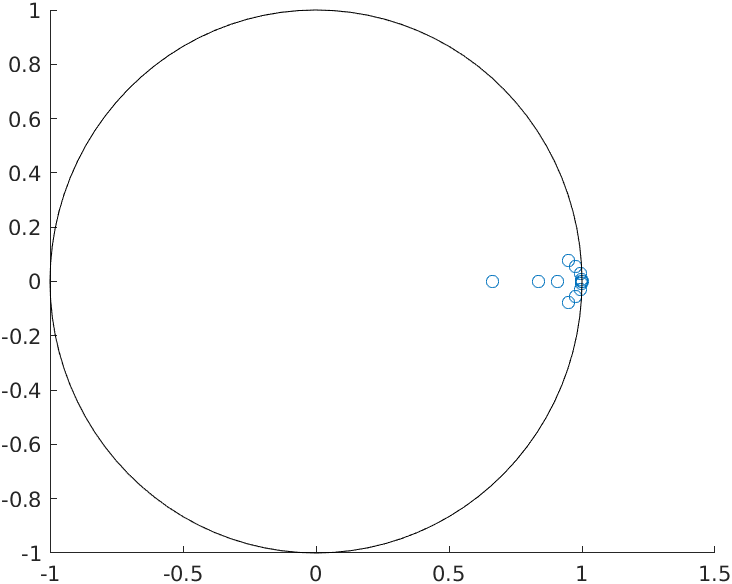
\includegraphics[width=\textwidth]{Steady_Eigen.png}
            \caption{Steady input eigenvalues}
            \label{fig:steady_eigen}
        \end{subfigure}
        \hfill
        \begin{subfigure}[b]{0.45\textwidth}
            \centering
            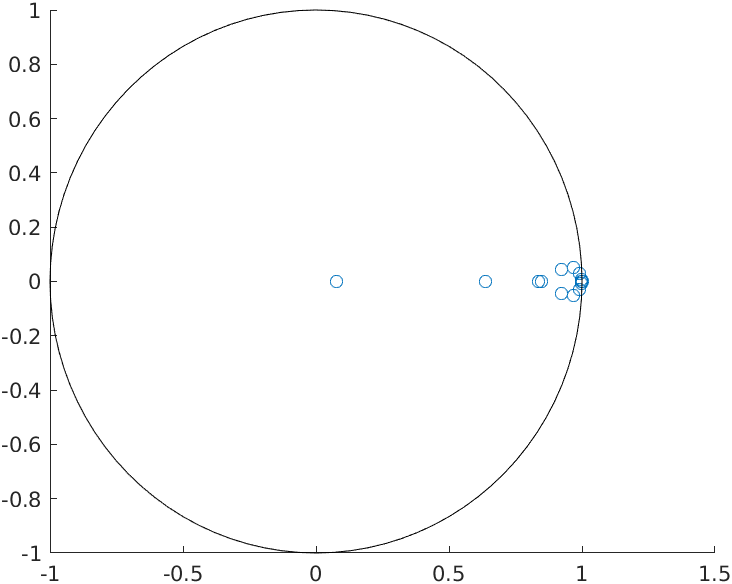
\includegraphics[width=\textwidth]{Unsteady_Eigen.png}
            \caption{Unsteady input eigenvalues}
            \label{fig:unsteady_eigen}
        \end{subfigure}
        \caption{Eigenvalues w.r.t. the Real-Imaginary unit circle}
        \label{fig:eigen}
    \end{figure}
\end{frame}


\section{Trajectory prediction}

\begin{frame}[fragile]{Training data - Visualization}
    \begin{lstlisting}[language=Matlab]
load(Data_Source+data(idx(1)).name);
i0 = 1; % Starting point
L = 3/0.02;

figure(2);
subplot(1,2,1);
scatter(z(1,:),z(2,:));
title("Original Data");
    \end{lstlisting}
\end{frame}

\begin{frame}[fragile]{Training data - Trajectory prediction}
    \begin{lstlisting}[language=Matlab]
g_p = zeros(size(g_t));
g_p(:,1) = Poly_Obs(z(:,i0),P,Nx,Nu);

for i=1:L
    g_p(:,i+1) = g_p(:,i)'*UN;

    % Input as data instead of prediction
    g_p(Nx+1:end,i+1) = z(Nx+1:end,i+1);
end

subplot(1,2,2);
scatter(g_p(2+P,:),g_p(2,:));
title("Trajectory Prediction");
    \end{lstlisting}
\end{frame}

\begin{frame}{Training data - Results}
    \begin{figure}
        \centering
        \begin{subfigure}[b]{0.45\textwidth}
            \centering
            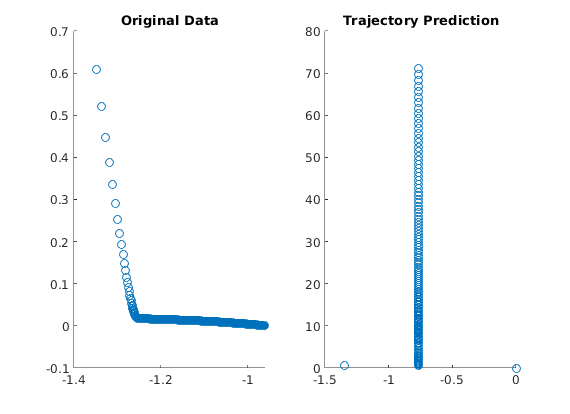
\includegraphics[width=\textwidth]{Steady_Verification.png}
            \caption{Steady input operator verification}
            \label{fig:steady_verify}
        \end{subfigure}
        \hfill
        \begin{subfigure}[b]{0.45\textwidth}
            \centering
            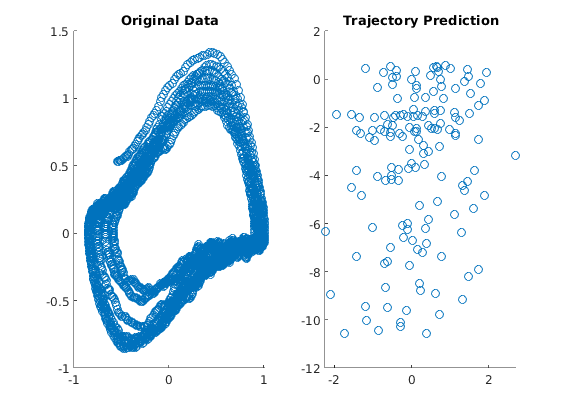
\includegraphics[width=\textwidth]{Unsteady_Verification.png}
            \caption{Unsteady input operator verification}
            \label{fig:unsteady_verify}
        \end{subfigure}
        \caption{Comparison between training trajectory and predicted trajectory}
    \end{figure}
\end{frame}

\begin{frame}[fragile]{New signal - Data generation}
    \begin{lstlisting}[language=matlab]
dt = 1e-2;
T = 20;

z0 = 4*rand(2,1) - 2;
sigma = randn(1);
u_t = 0:dt:T;
u = sigma * cos(u_t);

[t,z] = ode113(@(t,z) VanDerPol(t,z,u_t,u), u_t, z0);
z = [z';u];
L = length(0:dt:3);

figure(3);
subplot(1,2,1);
scatter(z(1,:),z(2,:));
title("New Simulation");
    \end{lstlisting}
\end{frame}

\begin{frame}[fragile]{New signal - Trajectory prediction}
    \begin{lstlisting}
g_p = zeros(size(g_t));
g_p(:,1) = Poly_Obs(z(:,i0),P,Nx,Nu);

for i=1:L
    g_p(:,i+1) = g_p(:,i)'*UN;
    g_p(Nx+1:end,i+1) = z(Nx+1:end,i+1);
end

subplot(1,2,2);
scatter(g_p(2+P,:),g_p(2,:));
title("Trajectory Prediction");
    \end{lstlisting}
\end{frame}

\begin{frame}{New signal - Results}
    \begin{figure}
        \centering
        \begin{subfigure}[b]{0.45\textwidth}
            \centering
            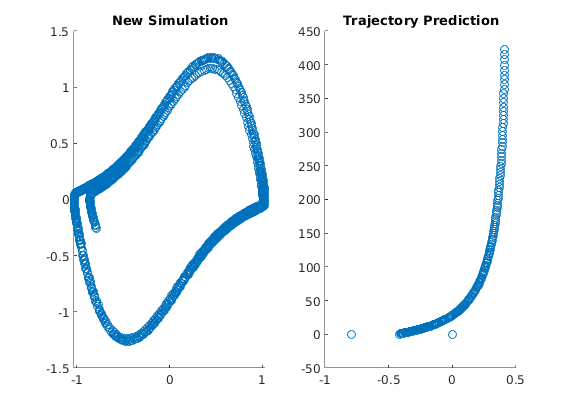
\includegraphics[width=\textwidth]{Steady_NewData.png}
            \caption{Steady input-trained new trajectory prediction}
            \label{fig:steady_new}
        \end{subfigure}
        \hfill
        \begin{subfigure}[b]{0.45\textwidth}
            \centering
            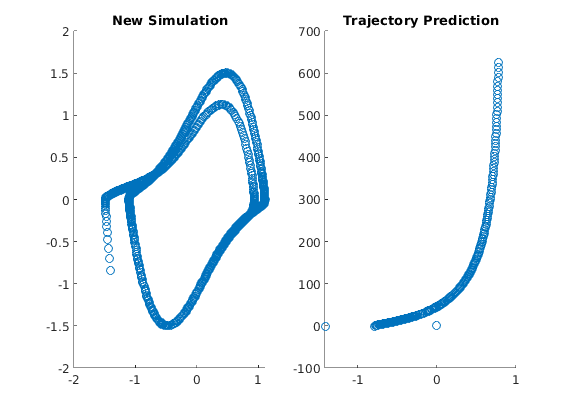
\includegraphics[width=\textwidth]{Unsteady_NewData.png}
            \caption{Unsteady input-trained new trajectory prediction}
            \label{fig:unsteady_new}
        \end{subfigure}
        \caption{Deterministic trajectory prediction test}
    \end{figure}
\end{frame}


\section{Conclusions}

\begin{frame}{Conclusions}
    \begin{itemize}
        \item Even if the results are unsatisfactory, Figure~\ref{fig:eigen} shows how a randomized input makes the eigenvalue associated to the input tend to 0, which is what we want for the final model.
        \item There must be an error in the process of prediction, since the magnitude of the eigenvalues clearly shows how the system should remain steady (or, at the very least, perpetually oscillating). As a consequence, I will resort to the base optimization process in order to recover the appropriate coefficients.
        \item Observing the simulated trajectories, we can see that the arbitrary input has been correctly integrated; this ensures that the prediction error comes from the later steps.
    \end{itemize}
\end{frame}

\end{document}